%% =============================================================================
%% APPENDIX - End-to-end evaluation protocol
%% =============================================================================

\section{End-to-end evaluation protocol} \label{app:e2e-eval}
\setcounter{table}{0}
\setcounter{figure}{0}

This appendix provides full protocol details for the end-to-end evaluation
reported in Section~\ref{sec:evaluation}.  The automated evaluation harness
drives the live \pkg{prompt2analytics} HTTP backend, loading datasets,
sending prompts at varying clarity levels, and scoring complete responses
including tool calls and LLM interpretations.  Complete prompts and scoring
data are provided in the supplementary materials.

\subsection{Models}

Table~\ref{tab:e2e-models} lists the six models evaluated, spanning
frontier cloud, efficient cloud, and open-source deployment scenarios.

\begin{table}[htbp]
\centering
\begin{threeparttable}
\caption{Models evaluated in end-to-end testing}
\label{tab:e2e-models}
\small
\begin{tabular}{llll}
\toprule
Model & Provider & Purpose & Parameters \\
\midrule
GPT-4.1 Mini      & OpenRouter (OpenAI) & Frontier cloud   & undisclosed \\
Claude Sonnet 4.6 & Anthropic API & Balanced cloud         & undisclosed \\
Claude Haiku 4.5  & Anthropic API & Fast cloud             & undisclosed \\
Gemini 2.5 Flash  & OpenRouter (Google) & Fast cloud        & undisclosed \\
Ministral 3B      & OpenRouter    & Minimal open-source    & 3B \\
Llama 4 Scout     & OpenRouter (Meta) & Open-source MoE    & 17B active (109B total) \\
\bottomrule
\end{tabular}
\begin{tablenotes}[flushleft]
\item \emph{Note:} All models accessed via API at temperature~$=0$.
Open-source models (Ministral~3B, Llama~4~Scout) can alternatively be
served locally via Ollama.  Tool definitions auto-generated from MCP
router schemas (119~Tier-1 tools).
\end{tablenotes}
\end{threeparttable}
\end{table}

\subsection{Synthetic datasets}

Six datasets with known data-generating processes provide ground-truth
parameters for scoring. Table~\ref{tab:e2e-datasets} summarises each dataset.

\begin{table}[htbp]
\centering
\begin{threeparttable}
\caption{Synthetic evaluation datasets}
\label{tab:e2e-datasets}
\small
\begin{tabular}{llrl}
\toprule
Dataset & Type & $n$ & Key DGP features \\
\midrule
\code{eval\_cross\_section} & Cross-section & 500 &
  $\text{salary} = 25000 + 3000 \cdot \text{edu} + 1500 \cdot \text{exp} + 500 \cdot \text{edu} \times \text{exp} + \varepsilon$ \\
\code{eval\_panel} & Panel ($N{=}50$, $T{=}10$) & 500 &
  Firm and year FEs; $\beta_{\text{value}} = 0.1$, $\beta_{\text{capital}} = 0.05$ \\
\code{eval\_timeseries} & Time series & 200 &
  AR(2) with $\phi_1{=}0.6$, $\phi_2{=}{-}0.2$; trend; seasonal \\
\code{eval\_treatment} & Treatment & 2000 &
  ATT${} = 3.0$; confounding via $x_1$, $x_2$; 2-period DiD structure \\
\code{eval\_messy} & Messy data & 300 &
  Coded names; $-99$ sentinels; \code{"N/A"} strings; mixed date formats \\
\code{eval\_survey} & Survey & 400 &
  Ordinal, binary, count outcomes; logit/probit/Poisson DGPs \\
\bottomrule
\end{tabular}
\begin{tablenotes}[flushleft]
\item \emph{Note:} All datasets generated with \code{set.seed(42)} in
\proglang{R}. True parameter values are documented in \code{PROTOCOL.md}.
\end{tablenotes}
\end{threeparttable}
\end{table}

\subsection{Test design}

Table~\ref{tab:e2e-tests} summarises the test structure. Each of 32~core tests
is written at three \emph{clarity levels}: precise (names the exact method and
all parameters), moderate (describes the goal without naming the method), and
vague (loose natural language). This yields 96 single-turn prompts.

\begin{table}[htbp]
\centering
\begin{threeparttable}
\caption{Test categories and counts}
\label{tab:e2e-tests}
\small
\begin{tabular}{lrrr}
\toprule
Category & Tests & Clarity levels & Total prompts \\
\midrule
Regression          & 5 & 3 & 15 \\
Panel data          & 4 & 3 & 12 \\
Causal inference    & 5 & 3 & 15 \\
Time series         & 4 & 3 & 12 \\
Hypothesis testing  & 4 & 3 & 12 \\
Discrete choice     & 3 & 3 &  9 \\
Machine learning    & 3 & 3 &  9 \\
Messy data          & 4 & 3 & 12 \\
\midrule
\textbf{Total}      & \textbf{32} & & \textbf{96} \\
\bottomrule
\end{tabular}
\begin{tablenotes}[flushleft]
\item \emph{Note:} Full prompts for all 96~tests are in
\code{test\_cases.json}.
\end{tablenotes}
\end{threeparttable}
\end{table}

\subsection{Scoring rubric}

Each prompt is scored on four dimensions (Table~\ref{tab:e2e-rubric}).
A prompt is classified as \emph{adequate} if it scores $\geq 62.5\%$ of the
applicable maximum (5/8 for numeric tasks, 4/6 when numerical correctness
is N/A).

\begin{table}[htbp]
\centering
\begin{threeparttable}
\caption{End-to-end scoring rubric}
\label{tab:e2e-rubric}
\small
\begin{tabular}{lp{9cm}}
\toprule
Dimension (0--2 each) & Scoring criteria \\
\midrule
Tool selection &
  2 = exact correct tool; 1 = acceptable alternative; 0 = wrong tool or no tool call \\
Parameter extraction &
  2 = all parameters correct; 1 = core parameters correct, optional missing;
  0 = wrong core parameters \\
Numerical correctness &
  2 = within tolerance of true DGP values; 1 = correct sign and magnitude;
  0 = wrong; N/A for non-numeric tasks \\
Interpretation quality &
  2 = accurate with context; 1 = superficial but correct; 0 = misleading \\
\bottomrule
\end{tabular}
\begin{tablenotes}[flushleft]
\item \emph{Note:} Maximum 8 points for numeric tasks, 6 for non-numeric.
Adequate threshold: $\geq 62.5\%$ of applicable maximum.
\end{tablenotes}
\end{threeparttable}
\end{table}

\subsection{Results by category}

Table~\ref{tab:e2e-category} shows the adequate rate by test category and
model.  All scores use auto-generated tool schemas from the MCP router
and the v2 evaluation harness with corrected parameter name matching.
Hypothesis testing achieves 100\% across the top four models.
ML tasks are uniformly strong due to simpler parameter schemas.
Causal inference shows the widest variation (60--93\%), reflecting
the difficulty of distinguishing between IPW, matching, and DiD designs.

\begin{table}[htbp]
\centering
\begin{threeparttable}
\caption{Adequate rate (\%) by category and model}
\label{tab:e2e-category}
\small
\begin{tabular}{lrrrrrr}
\toprule
Category & \rotatebox{60}{GPT-4.1 Mini} & \rotatebox{60}{Sonnet 4.6} & \rotatebox{60}{Haiku 4.5} & \rotatebox{60}{Ministr.\ 3B} & \rotatebox{60}{Gemini 2.5 Fl.} & \rotatebox{60}{Llama 4 Sc.} \\
\midrule
Hypothesis testing  & 100 & 100 & 100 &  75 & 100 &  75 \\
Time series         & 100 & 100 &  92 & 100 &  67 &  42 \\
Causal inference    &  93 &  73 &  33 &  87 &  60 &  60 \\
Panel data          &  92 &  75 & 100 &  75 &  75 &  58 \\
ML                  &  89 &  78 &  89 &  78 &  89 &  67 \\
Discrete choice     &  78 &  78 &  89 &  78 &  56 &  22 \\
Regression          &  87 &  80 &  80 &  87 &  73 &  33 \\
Messy data          &  83 &  92 &  83 &  58 &  83 &  42 \\
\bottomrule
\end{tabular}
\begin{tablenotes}[flushleft]
\item \emph{Note:} Adequate $= \geq 62.5\%$ of maximum score per prompt.
Each category has 9--15 prompts (3 clarity levels per test case).
Tool definitions auto-generated from MCP router schemas (119 Tier-1
tools).
\end{tablenotes}
\end{threeparttable}
\end{table}

\subsection{Chrome multi-turn evaluation details}

The Chrome-based evaluation drives the deployed Dioxus web frontend through
automated browser interaction, testing the full pipeline including SSE
streaming, session state management, and multi-turn context.  Eight
conversations with Claude Sonnet~4.6 cover the following workflows:

\begin{enumerate}
\item \textbf{MT1}: OLS regression $\to$ HC1 robust SEs $\to$ residual diagnostics (3 turns)
\item \textbf{MT2}: Panel data description $\to$ FE $\to$ Hausman test $\to$ RE (4 turns)
\item \textbf{MT3}: Time series description $\to$ stationarity tests $\to$ ARIMA $\to$ forecast (4 turns)
\item \textbf{MT4}: Naive OLS $\to$ DiD $\to$ balance check $\to$ IPW $\to$ comparison (5 turns)
\item \textbf{MT5}: Data quality assessment $\to$ sentinel replacement $\to$ renaming $\to$ regression (4 turns)
\item \textbf{MT6}: Survey data description $\to$ logit $\to$ ordered logit $\to$ negative binomial (4 turns)
\item \textbf{MT7}: OLS $\to$ diagnostic tests $\to$ specification choice (3 turns)
\item \textbf{MT8}: Cross-section OLS $\to$ panel FE $\to$ $R^2$ comparison (3 turns)
\end{enumerate}

\noindent Figure~\ref{fig:e2e-chrome-scores} shows per-conversation scores.
Five of eight conversations achieve perfect scores.  The three imperfect
conversations lose points to: data type casting limitations (MT5), superficial
interpretation of confounding (MT4), and ordered logit convergence with
unscaled predictors (MT6).

\begin{figure}[htbp]
\centering
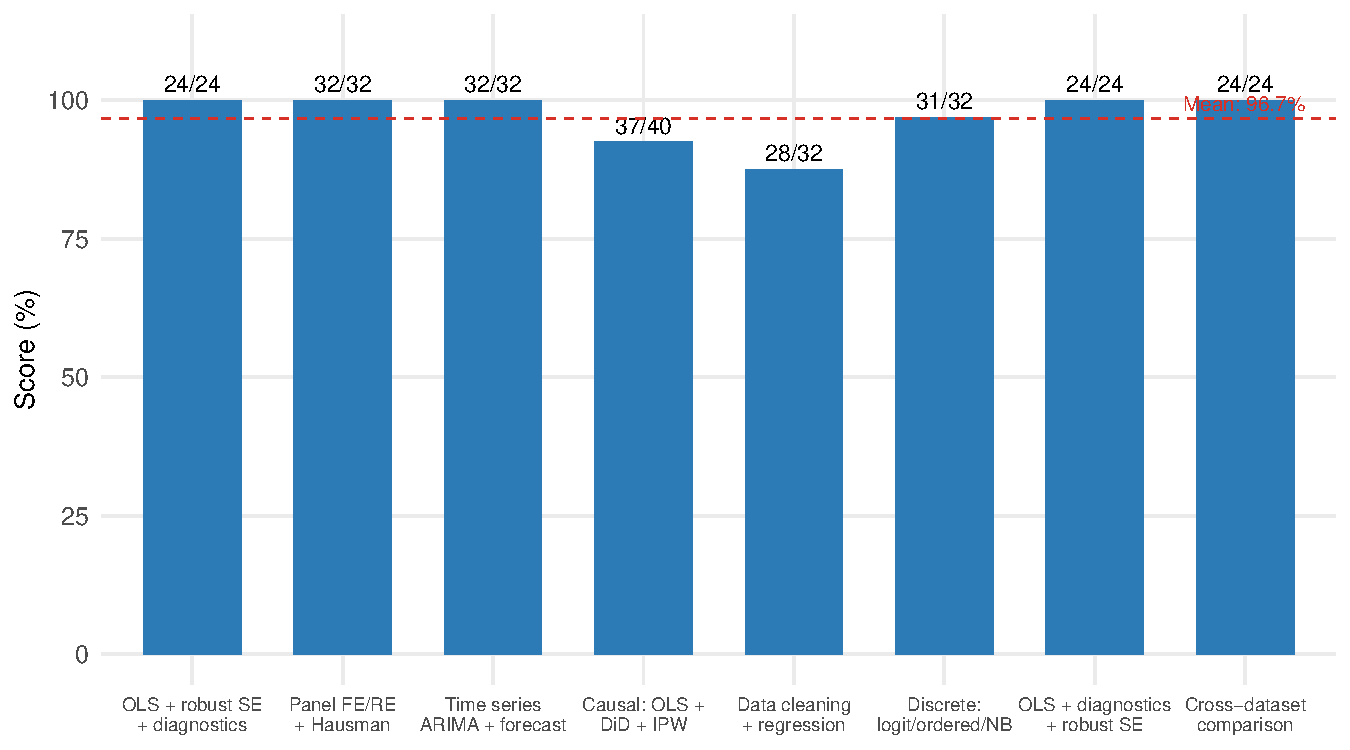
\includegraphics[width=0.95\textwidth]{figures/e2e_chrome_mt_scores}
\caption{Per-conversation scores in Chrome multi-turn evaluation
(Claude Sonnet~4.6). Dashed line shows overall mean (97.9\%).}
\label{fig:e2e-chrome-scores}
\end{figure}

\noindent Figure~\ref{fig:e2e-dimensions} shows per-dimension averages.
Tool selection and parameter extraction are perfect; numerical
correctness (1.77/2.00) is the primary source of lost points, driven
by tool limitations rather than model errors.

\begin{figure}[htbp]
\centering
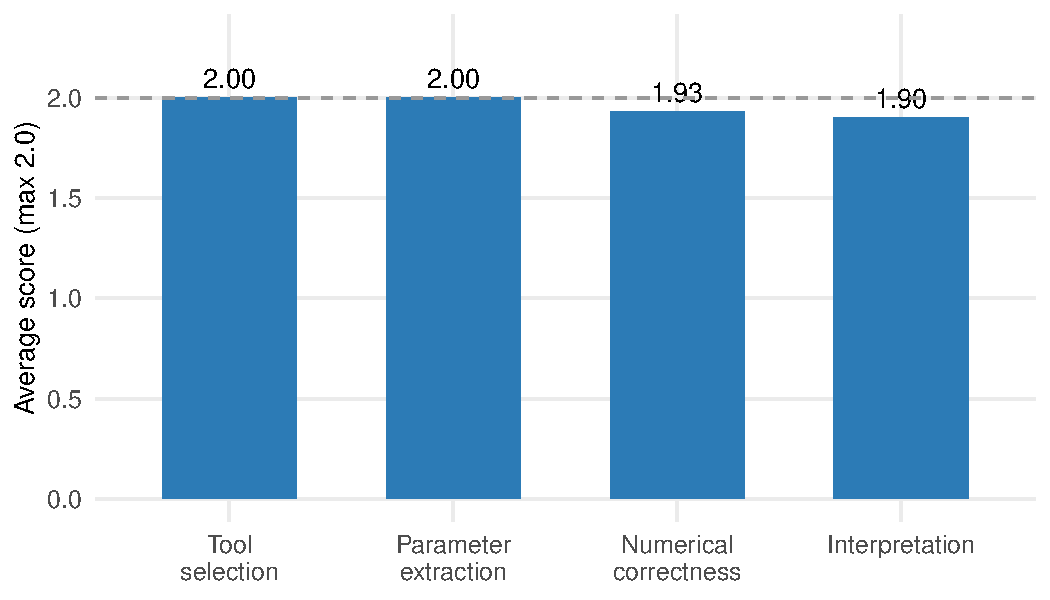
\includegraphics[width=0.75\textwidth]{figures/e2e_dimension_scores}
\caption{Per-dimension scoring averages across 30 turns
(Claude Sonnet~4.6, Chrome evaluation).}
\label{fig:e2e-dimensions}
\end{figure}

\subsection{Supplementary materials}

The complete evaluation materials are in \code{paper/code/e2e\_eval/}:
\code{PROTOCOL.md} (full protocol), \code{test\_cases.json} (all prompts with
expected tools and parameters), \code{generate\_datasets.R} (dataset DGPs),
\code{run\_evaluation.py} (automated evaluation harness),
\code{generate\_e2e\_figures.R} (figure and table generation from results),
and \code{results/} (raw scoring data in JSON format for all six models,
plus Chrome multi-turn results).
